\section{Corvilus}\label{corvilus}

Tags: razza

Nel fervore della battaglia, tutto sembra perduto. Guardi intorno, i
tuoi compagni sono caduti, il nemico sta marciando costantemente verso
di te e sai che il tuo tempo è giunto. Improvvisamente si fermano, le
bocche spalancate, fissando in lontananza. Giri la testa nel miglior
modo possibile e vedi una grande figura nera che vola attraverso il
cielo, librando verso di te. La figura atterra e inizia a colpire le
forze nemiche. Li spazza a destra e sinistra, facendoli scontrare gli
uni contro gli altri. Coloro che non sono sconfitti si ritirano dal
mostro che ti ha salvato. Guarda verso il cielo e emette un ruggito di
battaglia feroce.

\begin{figure}
\centering
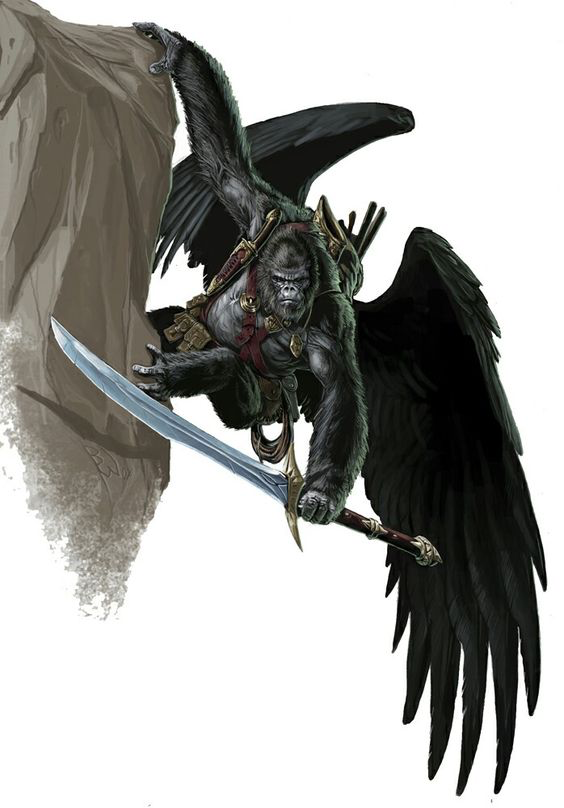
\includegraphics{Untitled 1.png}
\caption{Untitled}
\end{figure}

In una piccola capanna di montagna, una grande creatura nera è
accoccolata su un libro che sembra piccolo tra le sue mani. Sorride e
afferra una bacchetta alla sua destra. Agitando la bacchetta e
pronunciando le parole magiche, una scarica di fulmini erompe dalla
punta della bacchetta. La creatura ride e chiude il libro.

Camminando per le strade della tua città, vedi una grande figura. Sembra
una scimmia, ma è alta oltre tre metri. Cammina come un uomo che ha
perso tutto, è depresso con le lacrime agli occhi. Mentre ti passa
accanto, vedi due grandi cicatrici lungo la sua schiena, quasi come se
qualcosa fosse stato tagliato dalla sua pelle.

Queste grandi creature originano dal Piano Elementale dell'Aria ma lo
hanno abbandonato per il Piano Materiale dopo gli eventi della Grande
Tragedia.

\subsection{Descrizione fisica}\label{descrizione-fisica}

I Corivilus somigliano ai grandi gorilla dal dorso argentato della
Terra, ma hanno una differenza distintiva; possiedono due grandi ali,
situate sulla loro schiena. Alti oltre nove piedi, con un'apertura alare
media di venti piedi, questa razza è una forza con cui fare i conti.
Hanno due corte gambe simili a braccia nella parte inferiore del torso e
due lunghi bracci nella parte superiore. Hanno due mani e due piedi alle
estremità delle loro appendici, tutte dotate di pollici opponibili.
Hanno un volto e una testa distintamente simili a quelli delle scimmie.
A differenza delle altre scimmie, ma come gli umani, i Corivilus possono
scegliere di radere il viso o di far crescere una barba, baffi, basette
o tutto quanto sopra. L'intera superficie del loro corpo è coperta da
una folta pelliccia nera, ad eccezione delle mani, del viso e dello
stomaco, mentre le ali sono ricoperte di piume. Grazie alla loro folta
pelliccia e alla pelle spessa, indossano abiti minimi, anche nei luoghi
più freddi. Portano sempre un perizoma o una gonna per coprire i
genitali, ma principalmente indossano indumenti simili a cinture
utilitarie per contenere attrezzi e armi. Le femmine indossano un top
per coprire il seno, ma solo in presenza di altre razze. Un forestiero
che visita un villaggio di Corivilus troverebbe un villaggio con donne a
torso nudo.

\subsection{Storia}\label{storia}

I Corivilus vivevano una volta nel Piano Elementale dell'Aria, ma hanno
abbandonato la loro casa dopo La Grande Tragedia, in cui migliaia di
Corivilus furono massacrati dagli eserciti di Gargoyle. Da allora, si
sono rifugiati nel Piano Materiale, dove abitano nelle montagne e nelle
aree aride, in alto sopra il suolo. Lottano per trovare un luogo che li
ricordi della loro casa originale. Anche se ora sono stati nel Piano
Materiale per alcuni secoli e alcuni stanno cominciando a dimenticare le
loro origini.

\subsection{Società}\label{societuxe0}

I Corivilus vivono in villaggi di piccole o medie dimensioni governati
da un capo tribù. A causa della loro posizione scelta, hanno pochissime
fattorie e devono fare affidamento sulla caccia e la ricerca di cibo.
Dopo la Grande Tragedia, sono diventati molto diffidenti e in alcuni
casi estremamente violenti verso le altre razze. Questo fatto ha aiutato
nella scelta del loro habitat, poiché molte altre razze non possono
raggiungere le cime delle montagne. A differenza di altre società, i
giovani Corivilus vengono allevati dai loro nonni, invece dei genitori.
Il compito dei genitori è cacciare, raccogliere e proteggere, mentre il
compito dei nonni è insegnare ai giovani i modi dei Corivilus.

I giovani Corivilus raggiungono l'età adulta dopo aver completato il
rito di passaggio all'età di 10 anni. In questo rito di passaggio, il
giovane Corivilus deve volare sulla montagna più alta della regione e
recuperare un fiore che cresce da un cespuglio piantato dagli anziani.
Se recuperano il fiore, viene trasformato in una pasta utilizzata come
inchiostro per un tatuaggio che tutti i Corivilus possiedono. Questo
tatuaggio varia in dimensioni, forma e stile a seconda della tribù di
provenienza di un Corvilius, ma ha sempre una stampa di mano incorporata
nel disegno, a simboleggiare le mani degli anziani che sostengono il
Corivilus appena maturo.

I Corivilus sono severi quanto sono forti, e il tradimento non può
essere scusato. Quando un Corivilus viene esiliato dalla loro tribù, è
l'onore più grande immaginabile. Parte di questo è perché i membri della
tribù taglieranno le ali al Corivilus esiliato. Il Corivilus viene poi
bandito a terra, senza più la possibilità di volare o riunirsi con i
propri simili. Il suo ritorno significherebbe una morte certa.

\subsubsection{\texorpdfstring{\textbf{Corivilus
Traits}}{Corivilus Traits}}\label{corivilus-traits}

The Corivilus are a flying ape-like creature originally from the
Elemental Plane of Air.

\textbf{\emph{\href{https://www.dandwiki.com/wiki/5e_SRD:About_Races\#Ability_Score_Increase}{Ability
Score
Increase}.}}~Your~\href{https://www.dandwiki.com/wiki/5e_SRD:Strength}{Strength}~score
increases by 2 and
your~\href{https://www.dandwiki.com/wiki/5e_SRD:Constitution}{Constitution}~score
by 1.

\textbf{\emph{\href{https://www.dandwiki.com/wiki/5e_SRD:About_Races\#Age}{Age}.}}~Corivilus
generally live to the age of 100.

\textbf{\emph{\href{https://www.dandwiki.com/wiki/5e_SRD:About_Races\#Alignment}{Alignment}.}}~Corvilivus
tend to lean towards chaotic at a young age and lawful at an elderly
age. However, with everything there are always exceptions.

\textbf{\emph{\href{https://www.dandwiki.com/wiki/5e_SRD:About_Races\#Size}{Size}.}}~You
stand over nine feet tall and have a massive wingspan. Your size is
Medium.

\textbf{\emph{\href{https://www.dandwiki.com/wiki/5e_SRD:About_Races\#Speed}{Speed}.}}~Your
base walking speed is 35 feet. Your flying speed is 30 feet.

\textbf{\emph{Blade Proficiency.}}~Your race uses blades as their main
weapon of choice. You are proficient with
the~\href{https://www.dandwiki.com/wiki/5e_SRD:Shortsword}{shortsword},~\href{https://www.dandwiki.com/wiki/5e_SRD:Rapier}{rapier},~\href{https://www.dandwiki.com/wiki/5e_SRD:Longsword}{longsword},~\href{https://www.dandwiki.com/wiki/5e_SRD:Scimitar}{scimitar}~and~\href{https://www.dandwiki.com/wiki/5e_SRD:Greatsword}{greatsword}

\textbf{\emph{Wings.}}~You have a flying speed of 30 feet. If you are
wearing armor you are not proficient in or any Medium or Heavy armor,
you may not fly.

\textbf{\emph{Big Belly.}}~Because of your great size, you must eat and
drink twice as much as a human or else suffer from the effects
of~\href{https://www.dandwiki.com/wiki/5e_SRD:Conditions\#Exhaustion}{exhaustion}.

\textbf{\emph{Thick Furred.}}~You are almost completely covered with
thick black fur and you're acclimated to high altitude, including
elevations above 20,000 feet. This thick fur makes you naturally adapted
to cold climates, as described in chapter 5 of the Dungeon Master's
Guide.

\textbf{\emph{\href{https://www.dandwiki.com/wiki/5e_SRD:About_Races\#Languages}{Languages}.}}~You
speak, read and write common and Auran
